\section{Solver Parameter Testing}

\begin{frame}{Ignition Tests}
\begin{itemize}
\item Detonations can be initialized several ways
\begin{itemize}
    \item high $T$ and $P$ reactant block
    \item high $T$ and $P$ inert (e.g. helium) block
    \item gradient ignition, shown by Towery \textit{et. al.} \cite{towery2}
\end{itemize}
\item Necessary to test before AMR testing began 
\end{itemize}    
\end{frame}

\begin{frame}{Block Ignition}
Block of reactants at 3000 K and 20 atm spanning 0.001 m:
\begin{figure}[]
\centering
\includegraphics[width=0.7\textwidth]{../figs/ignition/block.png}
%\caption{Block ignition method, seen on left side of domain, at t = 0 s}
%\label{fig:blockig}
\end{figure}%
Abandoned due to due instability in detonation initiation.
\end{frame}

\begin{frame}{Gradient Ignition}
Gradient spanning from 1200 K and 4 atm to 300 K and 1 atm over 0.01 m:
\begin{figure}[]
\centering
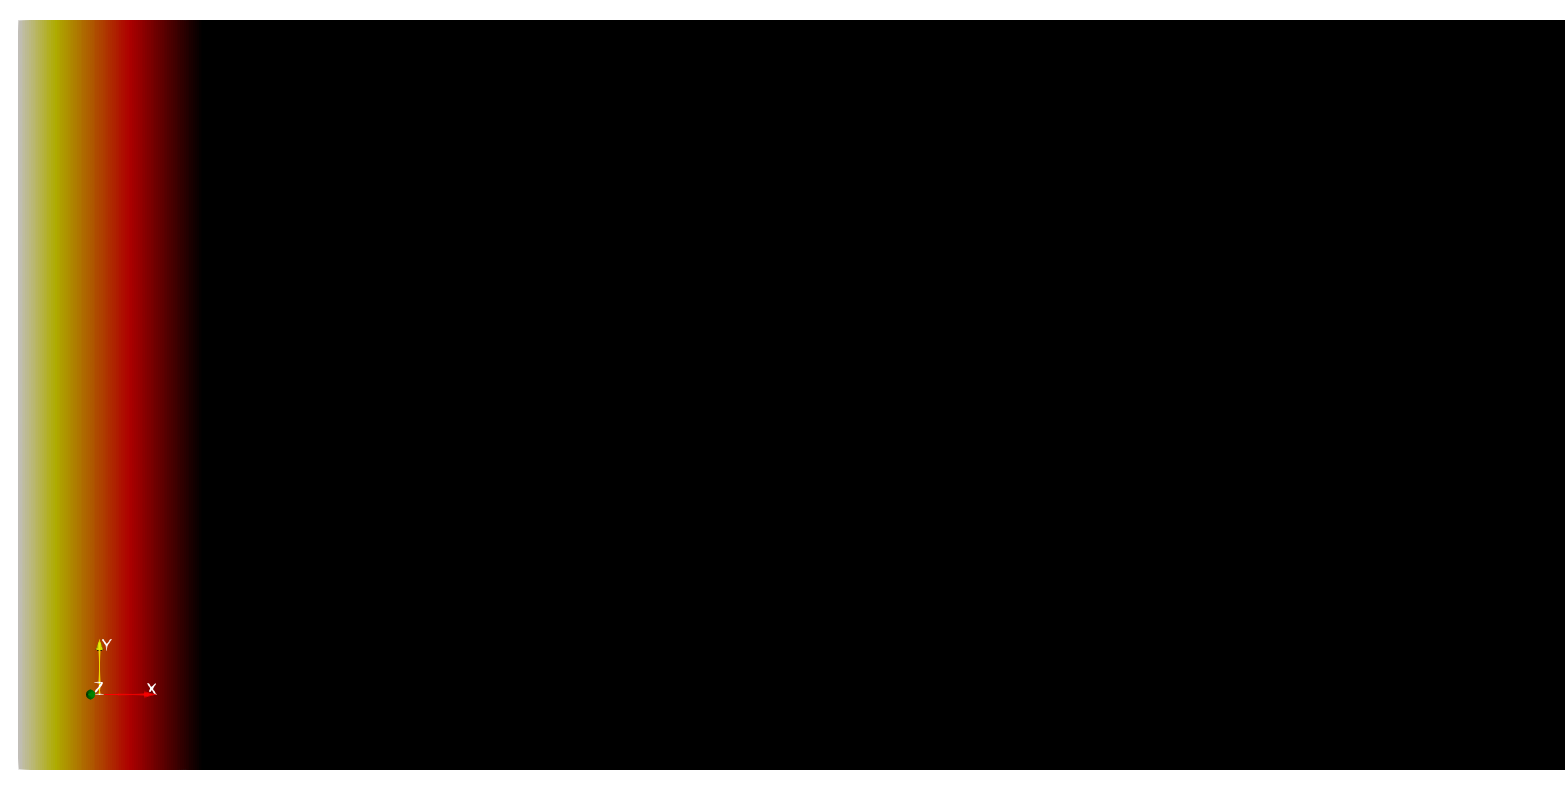
\includegraphics[width=0.7\textwidth]{../figs/ignition/gradient.png}
%\caption{Block ignition method, seen on left side of domain, at t = 0 s}
%\label{fig:blockig}
\end{figure}%
This produced smoother and more consistent detonations. 
\end{frame}

\begin{frame}{Cellular Detonation Modeling}
\begin{itemize}
\item Cellular ``fishscale'' patterns appear on smoked foils placed in detonation tube experiments
\item Can be used to verify numerical detonation modeling 
\item Numerical simulations can replicate this with maximum pressure and density traces over time for each cell
\item Temperature randomization was seeded throughout the domain, at up to 20\% of the maximum gradient temperature to assist cellular detonation formation 
\end{itemize}
\end{frame}

\begin{frame}{Cellular Detonation Modeling: Initial $T$ Randomization}
\begin{figure}[]
\centering
\includegraphics[width=\textwidth]{../figs/ignition/randgrad.png}
%\caption{Gradient ignition method with randomized temperature distribution throughout domain, seen on left side of domain, at t = 0 s}
%\label{fig:gradrand}
\end{figure}
\end{frame}

\begin{frame}{Cellular Detonation Modeling: Maximum $\rho$ Traces}
\begin{figure}[]
\centering
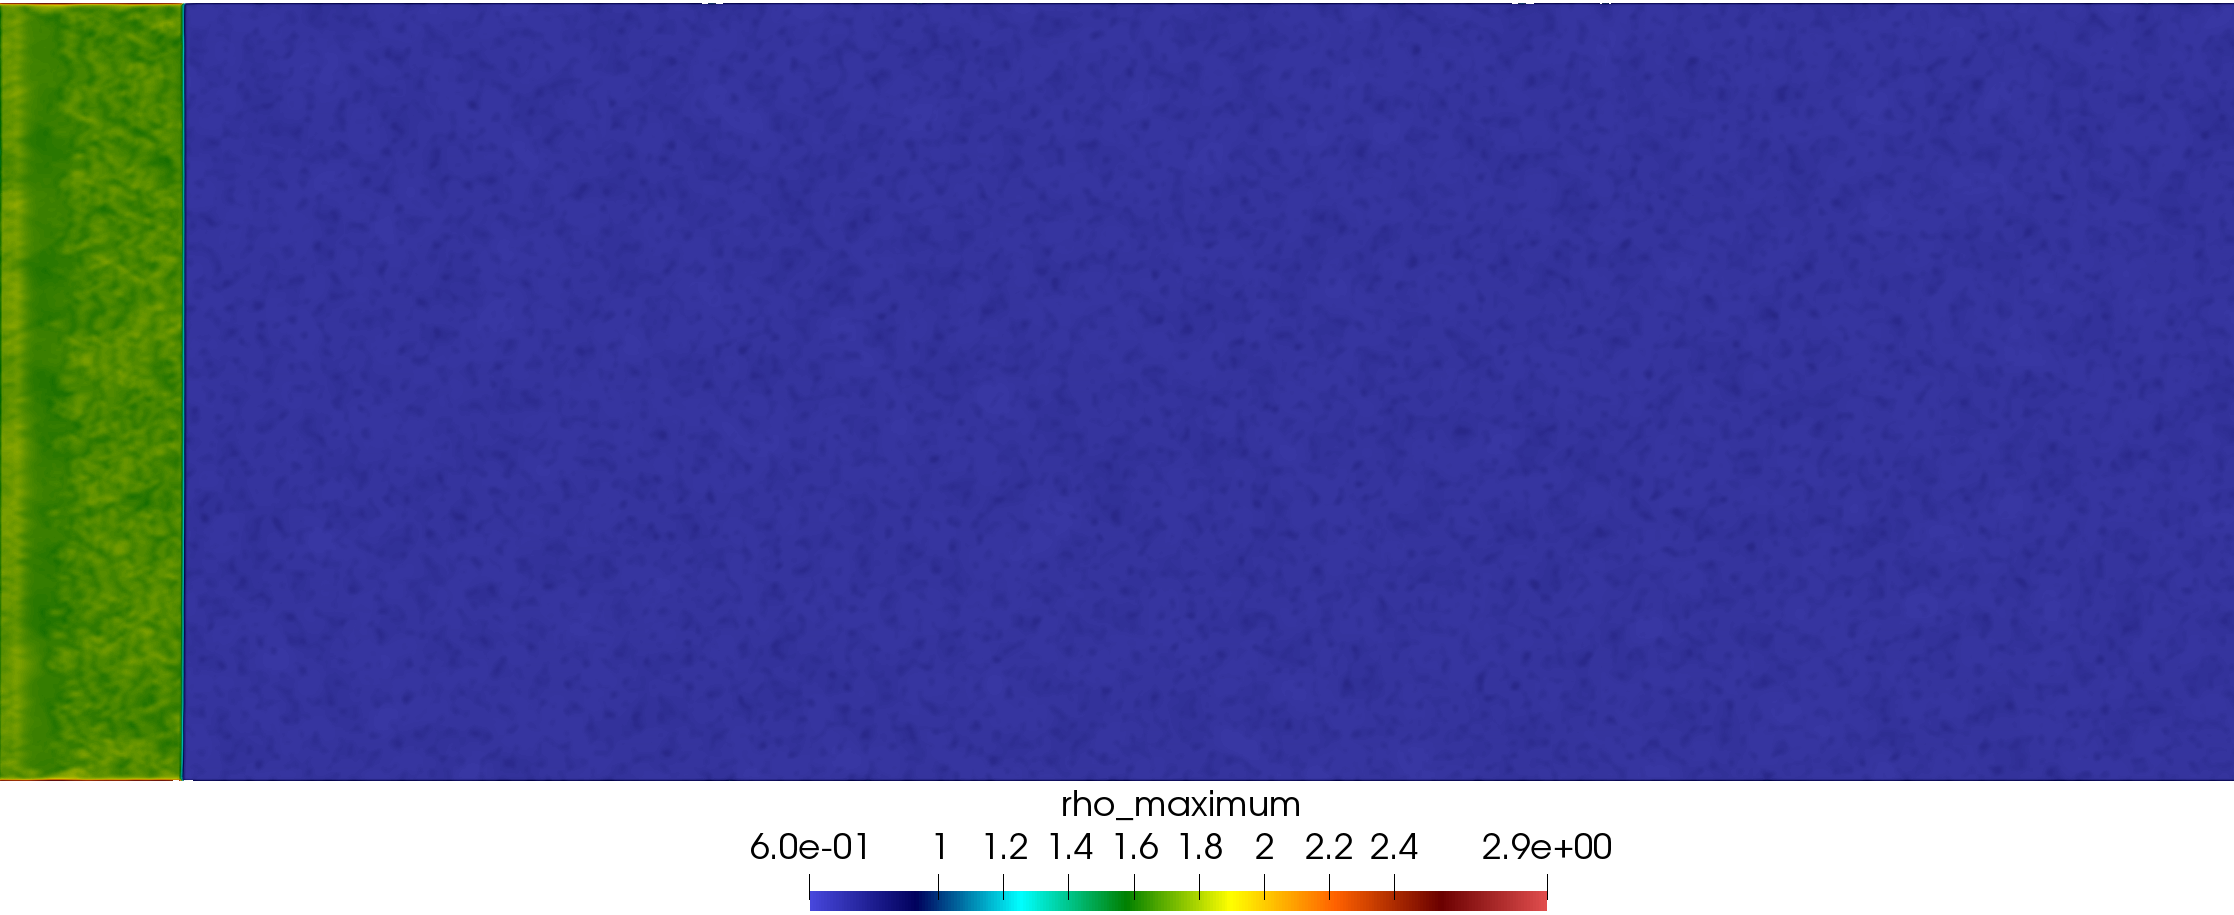
\includegraphics[width=\textwidth]{../figs/example_results/maxrho.png}
%\caption{Surface plot of maximum density tracked across all time steps for each cell, emulating a ``smoke foil''}
%\label{fig:maxrho}
\end{figure}
\end{frame}

\begin{frame}{Arrhenius Pre-exponential Factor $A$ Variation}
\begin{itemize}
\item Wanted to gauge sensitivity to Arrhenius pre-exponential factor as well as better match published values 
\item Swept exponent between $10^{11}$ and $10^{17}$ 
\item Plotted CJ target from similar setup by Towery \textit{et. al.} \cite{towery1}
\end{itemize}
\end{frame}

\begin{frame}{Arrhenius $A$ Variation: Pressure Distribution}
\begin{figure}
\centering
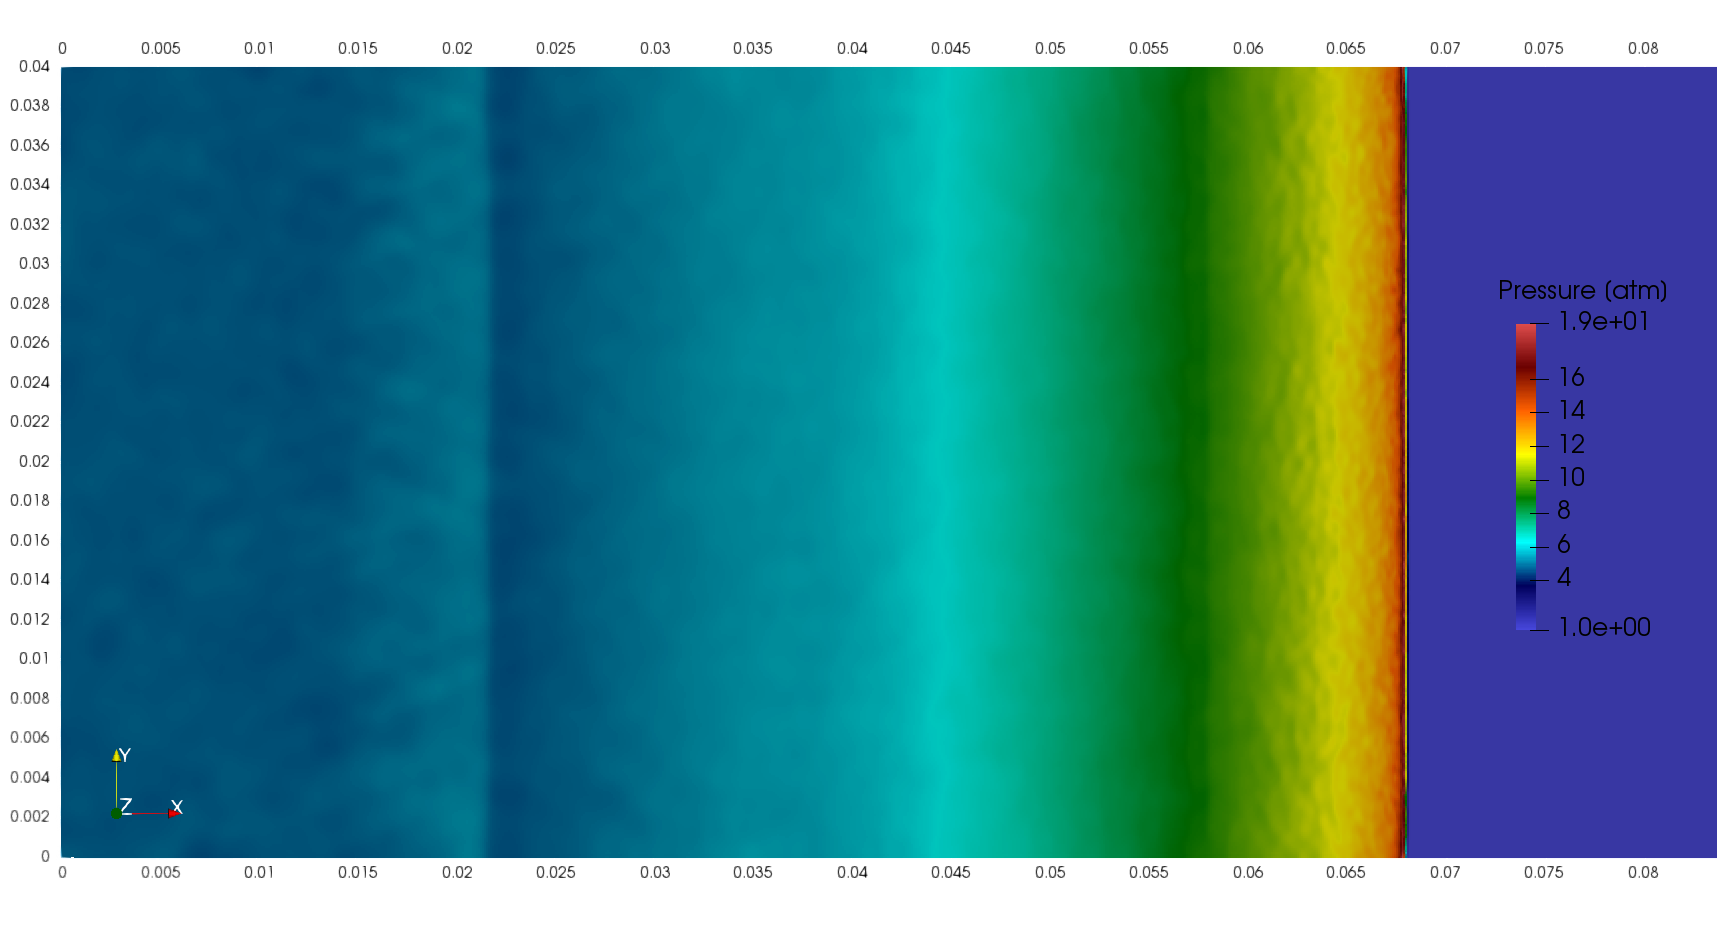
\includegraphics[width=0.8\linewidth]{../figs/Atest/p.png}
%\caption{Pressure distribution in detonation tube for pre-exponential factor exponent sweep test}
%\label{fig:atestp}
\end{figure}
\end{frame}

\begin{frame}{Arrhenius $A$ Variation: Temperature Distribution}
\begin{figure}
\centering
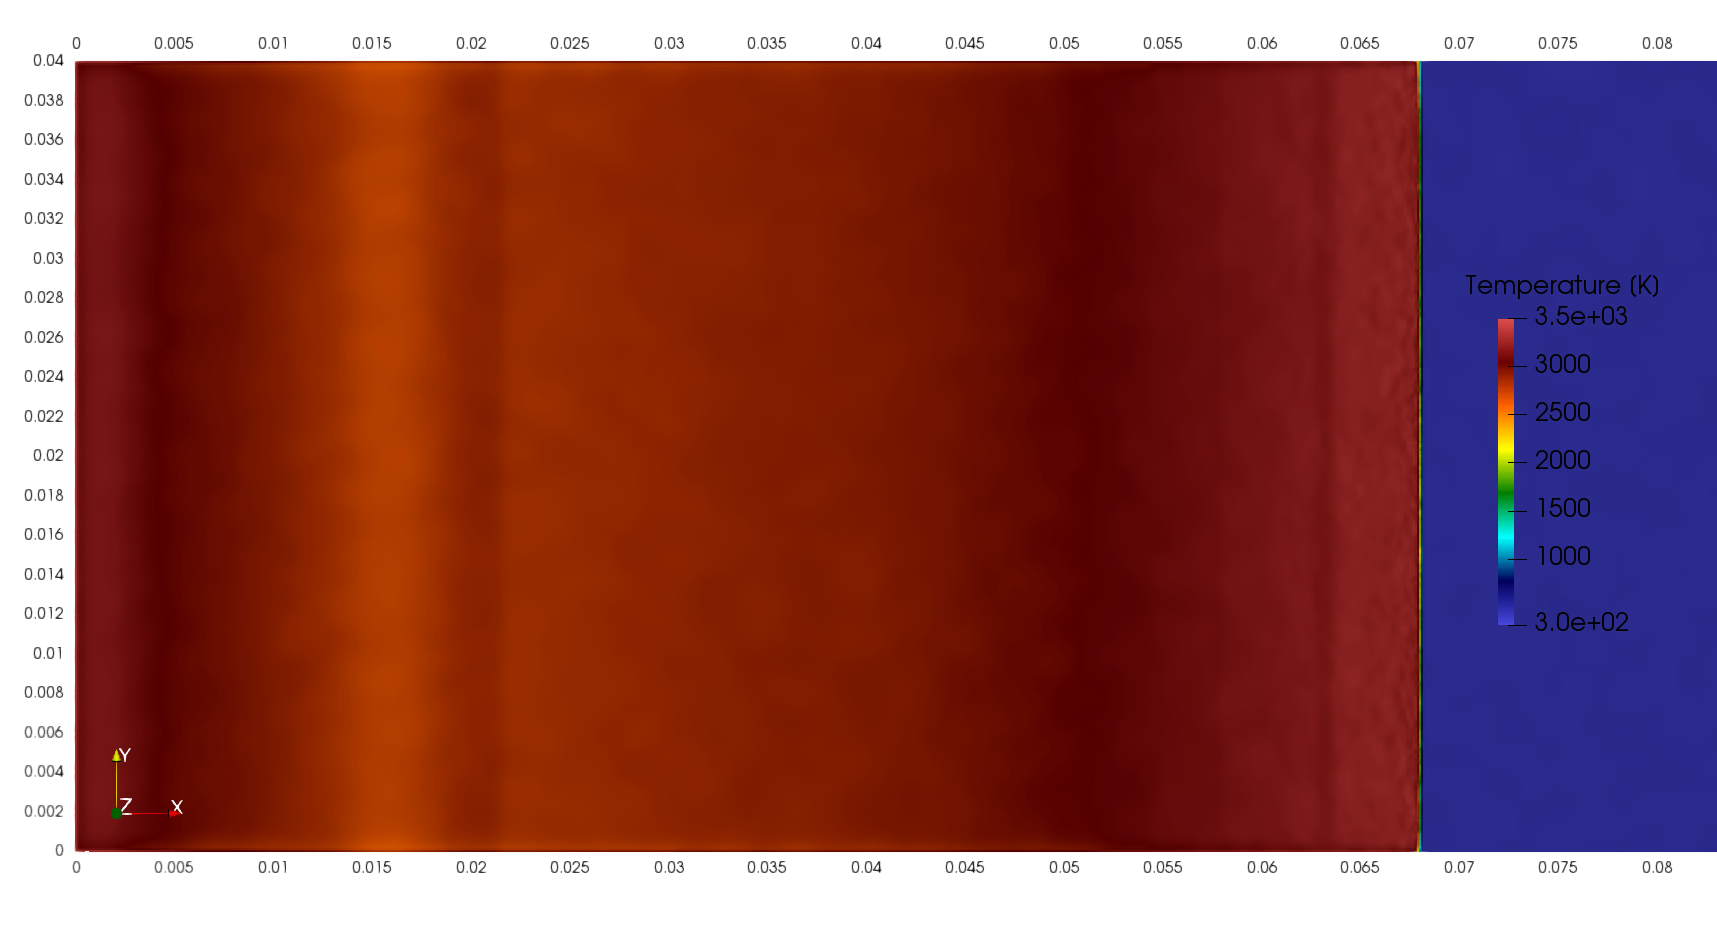
\includegraphics[width=0.8\linewidth]{../figs/Atest/t.png}
%\caption{Temperature distribution in detonation tube for pre-exponential factor exponent sweep test}
%\label{fig:atestt}
\end{figure}
\end{frame}

\begin{frame}{Arrhenius $A$ Variation: Velocity Distribution}
\begin{figure}
\centering
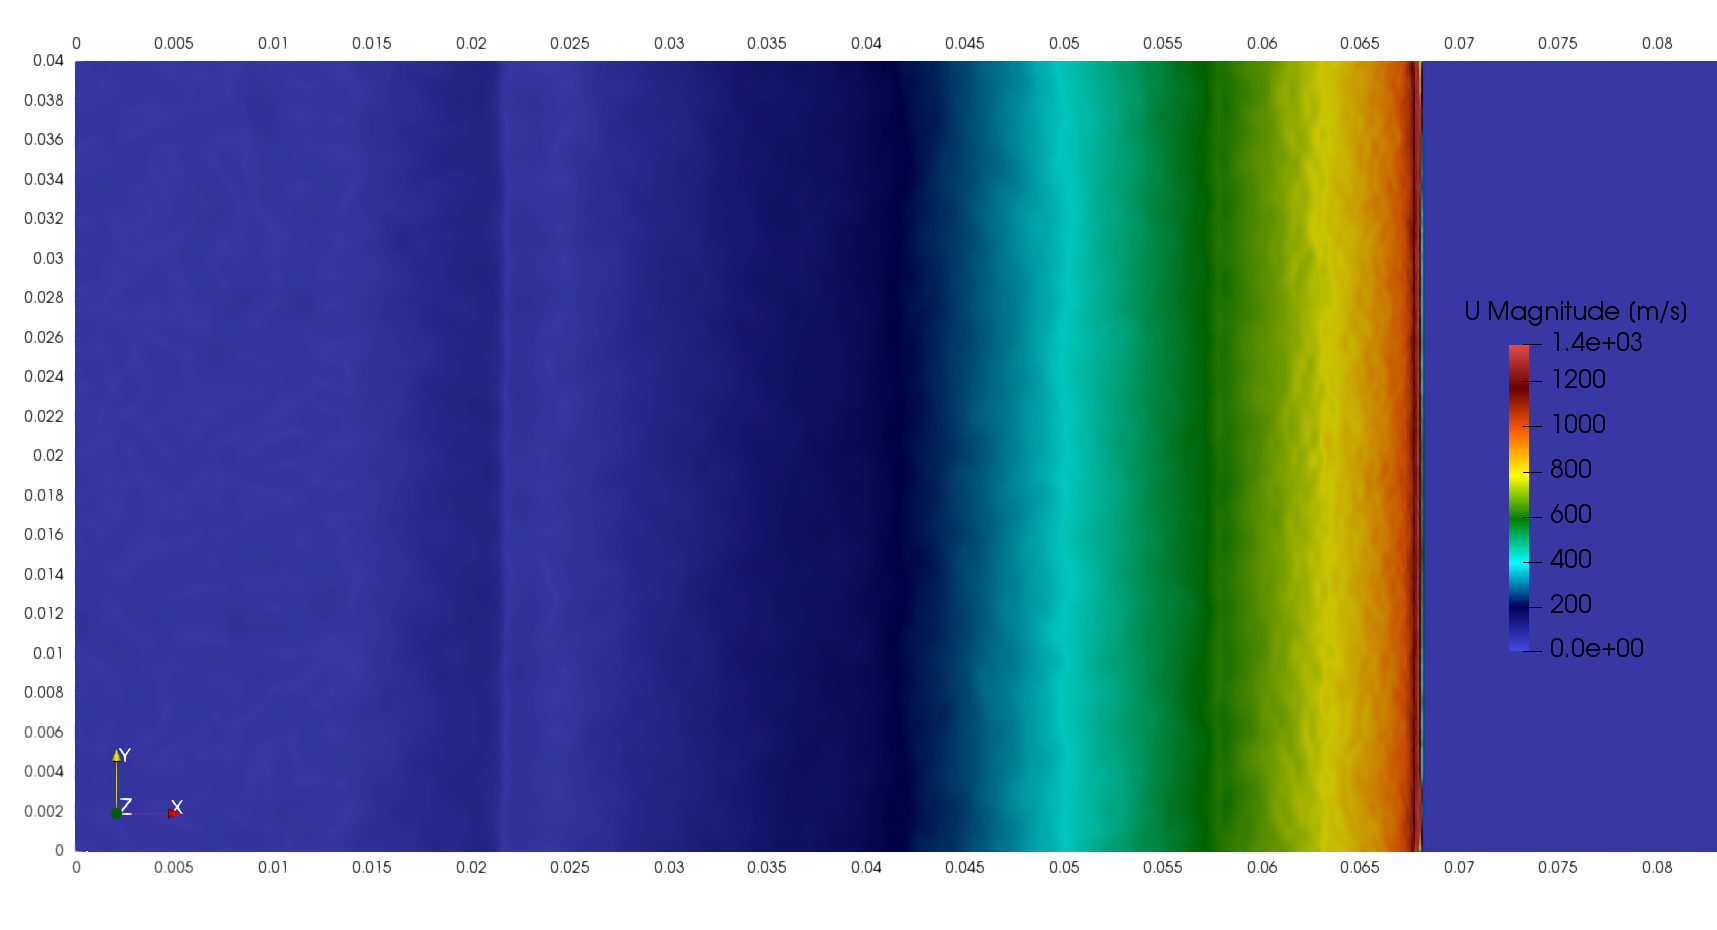
\includegraphics[width=0.8\linewidth]{../figs/Atest/u.png}
%\caption{Velocity distribution in detonation tube for pre-exponential factor exponent sweep test}
%\label{fig:atestu}
\end{figure}
\end{frame}


\begin{frame}{Arrhenius $A$ Variation: Detonation Decoupling}
\begin{figure}
\centering
\includegraphics[width=0.8\linewidth]{../figs/Atest_refined/p_large.png}
%\caption{Pressure distribution in detonation tube for expanded and refined pre-exponential factor exponent sweep test, showing detonation shock-reaction coupling transition. See Figures \ref{fig:atestrp} and \ref{fig:atestrt} for a filtered version.}
%\label{fig:pjump}
\end{figure}
\end{frame}



